\tikzset{every picture/.style={line width=0.75pt}} %set default line width to 0.75pt        

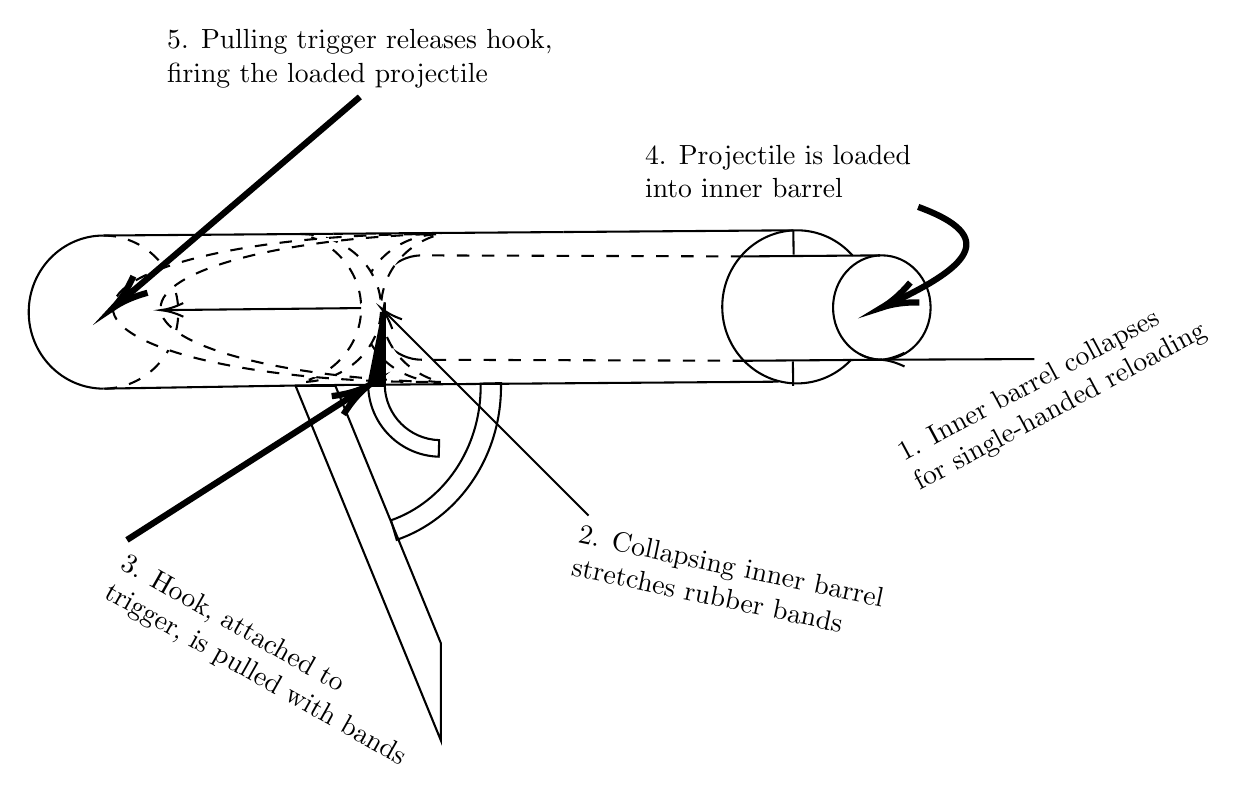
\begin{tikzpicture}[x=0.75pt,y=0.75pt,yscale=-1,xscale=1]
%uncomment if require: \path (0,471); %set diagram left start at 0, and has height of 471

%Shape: Diagonal Stripe [id:dp44643171889307887] 
\draw   (227.02,344.17) -- (227.02,391) -- (157.02,220.19) -- (176.21,220.19) -- cycle ;
%Shape: Arc [id:dp3829721896258529] 
\draw  [draw opacity=0][dash pattern={on 4.5pt off 4.5pt}] (64.5,147.79) .. controls (64.5,147.79) and (64.5,147.79) .. (64.5,147.79) .. controls (84.4,147.79) and (100.53,164.3) .. (100.53,184.67) .. controls (100.53,205.04) and (84.4,221.56) .. (64.5,221.56) -- (64.5,184.67) -- cycle ; \draw  [dash pattern={on 4.5pt off 4.5pt}] (64.5,147.79) .. controls (64.5,147.79) and (64.5,147.79) .. (64.5,147.79) .. controls (84.4,147.79) and (100.53,164.3) .. (100.53,184.67) .. controls (100.53,205.04) and (84.4,221.56) .. (64.5,221.56) ;  
%Straight Lines [id:da6447442957821032] 
\draw  [dash pattern={on 4.5pt off 4.5pt}]  (372.78,157.85) -- (217.1,157.36) ;
%Shape: Boxed Line [id:dp9137077542810423] 
\draw    (438.67,157.36) -- (372.78,157.85) ;
%Shape: Arc [id:dp31065750279651816] 
\draw  [draw opacity=0] (439.47,207.64) .. controls (426.5,207.63) and (415.99,196.37) .. (415.99,182.49) .. controls (415.99,168.92) and (426.04,157.86) .. (438.61,157.36) -- (439.49,182.49) -- cycle ; \draw   (439.47,207.64) .. controls (426.5,207.63) and (415.99,196.37) .. (415.99,182.49) .. controls (415.99,168.92) and (426.04,157.86) .. (438.61,157.36) ;  
%Shape: Arc [id:dp7246623187905588] 
\draw  [draw opacity=0] (437.77,157.41) .. controls (438.34,157.37) and (438.91,157.34) .. (439.49,157.34) .. controls (452.47,157.34) and (462.99,168.6) .. (462.99,182.49) .. controls (462.99,196.38) and (452.47,207.64) .. (439.49,207.64) .. controls (435.66,207.64) and (432.04,206.66) .. (428.84,204.91) -- (439.49,182.49) -- cycle ; \draw   (437.77,157.41) .. controls (438.34,157.37) and (438.91,157.34) .. (439.49,157.34) .. controls (452.47,157.34) and (462.99,168.6) .. (462.99,182.49) .. controls (462.99,196.38) and (452.47,207.64) .. (439.49,207.64) .. controls (435.66,207.64) and (432.04,206.66) .. (428.84,204.91) ;  
%Shape: Arc [id:dp8321391507112232] 
\draw  [draw opacity=0] (217.91,207.64) .. controls (204.94,207.63) and (194.43,196.37) .. (194.43,182.49) .. controls (194.43,168.92) and (204.48,157.86) .. (217.05,157.36) -- (217.93,182.49) -- cycle ; \draw   (217.91,207.64) .. controls (204.94,207.63) and (194.43,196.37) .. (194.43,182.49) .. controls (194.43,168.92) and (204.48,157.86) .. (217.05,157.36) ;  
%Shape: Arc [id:dp5772023197639267] 
\draw  [draw opacity=0] (424.79,207.52) .. controls (418.22,214.62) and (408.93,219.04) .. (398.63,219.04) .. controls (378.73,219.04) and (362.6,202.53) .. (362.6,182.16) .. controls (362.6,161.79) and (378.73,145.27) .. (398.63,145.27) .. controls (409.3,145.27) and (418.88,150.02) .. (425.48,157.55) -- (398.63,182.16) -- cycle ; \draw   (424.79,207.52) .. controls (418.22,214.62) and (408.93,219.04) .. (398.63,219.04) .. controls (378.73,219.04) and (362.6,202.53) .. (362.6,182.16) .. controls (362.6,161.79) and (378.73,145.27) .. (398.63,145.27) .. controls (409.3,145.27) and (418.88,150.02) .. (425.48,157.55) ;  
%Straight Lines [id:da8276168802295119] 
\draw    (439.47,207.64) -- (373.59,208.13) ;
%Straight Lines [id:da8086723755554028] 
\draw  [dash pattern={on 4.5pt off 4.5pt}]  (373.59,208.13) -- (217.91,207.64) ;
%Shape: Boxed Line [id:dp04417146350403023] 
\draw    (396.84,145.27) -- (286.06,146.11) ;
%Shape: Boxed Line [id:dp4650146603828804] 
\draw    (286.06,146.11) -- (175.28,146.95) ;
%Shape: Boxed Line [id:dp2321133945044378] 
\draw    (389.79,218.2) -- (279.01,219.04) ;
%Shape: Boxed Line [id:dp1511670848453761] 
\draw    (279.01,219.04) -- (168.23,219.88) ;
%Shape: Moon [id:dp8540543539810237] 
\draw  [fill={rgb, 255:red, 255; green, 255; blue, 255 }  ,fill opacity=1 ][dash pattern={on 4.5pt off 4.5pt}] (227.01,218.36) .. controls (205.81,218.36) and (188.63,202.41) .. (188.63,182.74) .. controls (188.63,163.06) and (205.81,147.11) .. (227.01,147.11) .. controls (210.44,151.21) and (198.22,165.61) .. (198.22,182.74) .. controls (198.22,199.87) and (210.44,214.27) .. (227.01,218.36) -- cycle ;
%Shape: Moon [id:dp5882029644966247] 
\draw  [fill={rgb, 255:red, 255; green, 255; blue, 255 }  ,fill opacity=1 ][dash pattern={on 4.5pt off 4.5pt}] (159.84,147.11) .. controls (181.04,147.11) and (198.22,163.06) .. (198.22,182.74) .. controls (198.22,202.41) and (181.04,218.36) .. (159.84,218.36) .. controls (176.41,214.27) and (188.63,199.87) .. (188.63,182.74) .. controls (188.63,165.61) and (176.41,151.21) .. (159.84,147.11) -- cycle ;
%Shape: Boxed Line [id:dp6579420712092399] 
\draw    (175.28,146.95) -- (64.5,147.79) ;
%Shape: Boxed Line [id:dp19771990599738065] 
\draw    (168.23,219.88) -- (64.5,221.56) ;
%Shape: Boxed Line [id:dp09246533962136039] 
\draw    (512.98,207.31) -- (441.47,207.63) ;
\draw [shift={(439.47,207.64)}, rotate = 359.74] [color={rgb, 255:red, 0; green, 0; blue, 0 }  ][line width=0.75]    (10.93,-3.29) .. controls (6.95,-1.4) and (3.31,-0.3) .. (0,0) .. controls (3.31,0.3) and (6.95,1.4) .. (10.93,3.29)   ;
%Curve Lines [id:da06123511321721531] 
\draw [line width=2.25]    (457,134) .. controls (496.77,148.55) and (481.03,163.1) .. (443.07,180.84) ;
\draw [shift={(439.49,182.49)}, rotate = 335.47] [color={rgb, 255:red, 0; green, 0; blue, 0 }  ][line width=2.25]    (17.49,-5.26) .. controls (11.12,-2.23) and (5.29,-0.48) .. (0,0) .. controls (5.29,0.48) and (11.12,2.23) .. (17.49,5.26)   ;
%Shape: Boxed Line [id:dp04823339202175414] 
\draw    (298.22,282.74) -- (199.64,184.15) ;
\draw [shift={(198.22,182.74)}, rotate = 45] [color={rgb, 255:red, 0; green, 0; blue, 0 }  ][line width=0.75]    (10.93,-3.29) .. controls (6.95,-1.4) and (3.31,-0.3) .. (0,0) .. controls (3.31,0.3) and (6.95,1.4) .. (10.93,3.29)   ;
%Shape: Moon [id:dp24174634531764227] 
\draw  [fill={rgb, 255:red, 255; green, 255; blue, 255 }  ,fill opacity=1 ][dash pattern={on 4.5pt off 4.5pt}] (221.01,218.36) .. controls (137.06,218.36) and (69,202.41) .. (69,182.74) .. controls (69,163.06) and (137.06,147.11) .. (221.01,147.11) .. controls (147.9,149.75) and (92,164.7) .. (92,182.74) .. controls (92,200.78) and (147.9,215.72) .. (221.01,218.36) -- cycle ;
%Shape: Boxed Line [id:dp9421913663732036] 
\draw    (188.63,182.74) -- (94,183.72) ;
\draw [shift={(92,183.74)}, rotate = 359.41] [color={rgb, 255:red, 0; green, 0; blue, 0 }  ][line width=0.75]    (10.93,-3.29) .. controls (6.95,-1.4) and (3.31,-0.3) .. (0,0) .. controls (3.31,0.3) and (6.95,1.4) .. (10.93,3.29)   ;
%Shape: Block Arc [id:dp2671154342059705] 
\draw   (225.99,254.35) .. controls (207.41,253.82) and (192.45,238.8) .. (192.02,220.19) -- (200,220) .. controls (200.33,234.37) and (211.88,245.96) .. (226.22,246.37) -- cycle ;
%Shape: Right Triangle [id:dp12222925013676056] 
\draw  [fill={rgb, 255:red, 0; green, 0; blue, 0 }  ,fill opacity=1 ] (200,180) -- (192.02,220.19) -- (200,220.19) -- cycle ;
%Straight Lines [id:da6026957076507713] 
\draw [line width=2.25]    (75.8,294.45) -- (188.65,222.34) ;
\draw [shift={(192.02,220.19)}, rotate = 147.42] [color={rgb, 255:red, 0; green, 0; blue, 0 }  ][line width=2.25]    (17.49,-5.26) .. controls (11.12,-2.23) and (5.29,-0.48) .. (0,0) .. controls (5.29,0.48) and (11.12,2.23) .. (17.49,5.26)   ;
%Straight Lines [id:da09418100379889882] 
\draw    (396.84,145.27) -- (397,157) ;
%Straight Lines [id:da8937010383750714] 
\draw    (396.63,208.48) -- (396.79,220.2) ;
%Shape: Arc [id:dp6616955505275475] 
\draw  [draw opacity=0] (64.5,221.56) .. controls (64.5,221.56) and (64.5,221.56) .. (64.5,221.56) .. controls (44.6,221.56) and (28.46,205.04) .. (28.46,184.67) .. controls (28.46,164.3) and (44.6,147.79) .. (64.5,147.79) -- (64.5,184.67) -- cycle ; \draw   (64.5,221.56) .. controls (64.5,221.56) and (64.5,221.56) .. (64.5,221.56) .. controls (44.6,221.56) and (28.46,205.04) .. (28.46,184.67) .. controls (28.46,164.3) and (44.6,147.79) .. (64.5,147.79) ;  
%Shape: Block Arc [id:dp10633354848632748] 
\draw   (256,218.92) .. controls (256.01,219.44) and (256.01,219.97) .. (256.01,220.5) .. controls (256.01,255.14) and (234.9,284.47) .. (205.77,294.4) -- (203,284.99) .. controls (228.07,276.25) and (246.21,250.68) .. (246.21,220.5) .. controls (246.21,220.04) and (246.21,219.59) .. (246.2,219.13) -- cycle ;
%Straight Lines [id:da8113082771754814] 
\draw [line width=2.25]    (188,81) -- (72.04,180.14) ;
\draw [shift={(69,182.74)}, rotate = 319.47] [color={rgb, 255:red, 0; green, 0; blue, 0 }  ][line width=2.25]    (17.49,-5.26) .. controls (11.12,-2.23) and (5.29,-0.48) .. (0,0) .. controls (5.29,0.48) and (11.12,2.23) .. (17.49,5.26)   ;

% Text Node
\draw (514.4,209.95) node [anchor=north] [inner sep=0.75pt]  [rotate=-331.77] [align=left] {1. Inner barrel collapses\\for single-handed reloading};
% Text Node
\draw (455,131) node [anchor=south east] [inner sep=0.75pt]   [align=left] {4. Projectile is loaded\\into inner barrel};
% Text Node
\draw (293.56,285.09) node [anchor=north west][inner sep=0.75pt]  [rotate=-11.92] [align=left] {2. Collapsing inner barrel\\stretches rubber bands};
% Text Node
\draw (76.06,298.05) node [anchor=north west][inner sep=0.75pt]  [rotate=-29.52] [align=left] {3. Hook, attached to \\trigger, is pulled with bands};
% Text Node
\draw (188,78) node [anchor=south] [inner sep=0.75pt]   [align=left] {5. Pulling trigger releases hook,\\firing the loaded projectile};


\end{tikzpicture}
